% AER-Article.tex for AEA last revised 22 June 2011
\documentclass[AER]{AEA}

% The mathtime package uses a Times font instead of Computer Modern.
% Uncomment the line below if you wish to use the mathtime package:
%\usepackage[cmbold]{mathtime}
% Note that miktex, by default, configures the mathtime package to use commercial fonts
% which you may not have. If you would like to use mathtime but you are seeing error
% messages about missing fonts (mtex.pfb, mtsy.pfb, or rmtmi.pfb) then please see
% the technical support document at http://www.aeaweb.org/templates/technical_support.pdf
% for instructions on fixing this problem.

% Note: you may use either harvard or natbib (but not both) to provide a wider
% variety of citation commands than latex supports natively. See below.

% Uncomment the next line to use the natbib package with bibtex
\usepackage{natbib}

% Uncomment the next line to use the harvard package with bibtex
%\usepackage[abbr]{harvard}

% This command determines the leading (vertical space between lines) in draft mode
% with 1.5 corresponding to "double" spacing.
\draftSpacing{1.5}


% tightlist command for lists without linebreak
\providecommand{\tightlist}{%
  \setlength{\itemsep}{0pt}\setlength{\parskip}{0pt}}

% From pandoc table feature
\usepackage{longtable,booktabs,array}
\usepackage{calc} % for calculating minipage widths
% Correct order of tables after \paragraph or \subparagraph
\usepackage{etoolbox}
\makeatletter
\patchcmd\longtable{\par}{\if@noskipsec\mbox{}\fi\par}{}{}
\makeatother
% Allow footnotes in longtable head/foot
\IfFileExists{footnotehyper.sty}{\usepackage{footnotehyper}}{\usepackage{footnote}}
\makesavenoteenv{longtable}


\usepackage{graphicx}
\usepackage{booktabs}

\usepackage{hyperref}

\begin{document}


\title{Comparing Global \(CO_{2}\) Emission Models from 1997 and Today}
\shortTitle{A comparative follow up report}
% \author{Author1 and Author2\thanks{Surname1: affiliation1, address1, email1.
% Surname2: affiliation2, address2, email2. Acknowledgements}}


\author{
  Carolyn Dunlap\\
  Ayda Nayeb Nazar\\
  Qian Qiao\\
  Hector Rincon\thanks{
  : , \href{mailto:}{}.
  : , \href{mailto:}{}.
  : , \href{mailto:}{}.
  : , \href{mailto:}{}.
  The authors would like to thank their instructors from MIDS 271.
}
}

\date{\today}
\pubMonth{03}
\pubYear{2023}
\pubVolume{0}
\pubIssue{0}
\JEL{}
\Keywords{Replication, Modern Science}

\begin{abstract}
In 1997, our team analyzed \(CO_{2}\) concentration avaerage monthly
trends from 1959 to 1997. Our work culminated in a report that discussed
multiple linear and ARIMA models of these concentration data and
attempted to forecast \(CO_{2}\) trends into the future, as far out as
2100. Given that we now have 25 more years of data, and at a highly
weekly resolution, this report aims to revisit and evaluate our 1997
models. Using weekly average \(CO_{2}\) concentration levels taking from
the Mauna Loa observatory, we also analyze our data to fit new models
and generate updated forcasts for potential \(CO_{2}\) concentrations as
far out as 100 years into the future.
\end{abstract}


\maketitle

\hypertarget{introduction}{%
\section{Introduction}\label{introduction}}

In this report, we are continuing to evaluate atmospheric \(CO_{2}\)
trends (commonly referred to as the Keeling Curve), generating models
and forecasts to help understand how we might expect atmospheric
\(CO_{2}\) levels to change in the future. Specifically, we are
re-evaluating our best performing linear and ARIMA models from our 1997
report on \(CO_{2}\) concentrations, using more recently generating
weekly average \(CO_{2}\) data up through the end of 2022. This report
continues to use the \(CO_{2}\) concentration data collected by the
Mauna Loa observatory, with the key exception that we have weekly
average \(CO_{2}\) concentration data, compared to the monthly average
concentration data used in 1997. Depending on the purposes of our
analyses, we will either keep the weekly granularity or regenerate
monthly averages as necessary. In addition to evaluating our 1997 models
and forecasts, we will also use more recent data to generate new models
and forecasts for \(CO_{2}\) concentrations.

\hypertarget{measurement-and-data}{%
\section{Measurement and Data}\label{measurement-and-data}}

The data that we are using from this report was accessed via the United
States' National Oceanic and Atmospheric Administration website, where
they house continually updated weekly \(CO_{2}\) concentration data
collected from the Mauna Loa observatory. This data was collected in a
similar manner to the data in 1997 with a few key exceptions.

The first key exception is that in 2019, the observatory installed a new
\(CO_{2}\) analyzer that measures \(CO_{2}\) concentration (defined as
the number of \(CO_{2}\) molecules out of a random million atmospheric
molecules, or parts per million (ppm)) via cavity-ring down spectroscopy
versus the previously used infrared absorption. We are presuming that
this change in analysis technique does not dramatically alter the
concentration of \(CO_{2}\). Another exception is that this dataset has
a gap in December 1975: for the purposes of these analyses, we decided
to fill all gaps using the previous \(CO_{2}\) concentration gathered
(e.g.~we decided to use the \(CO_{2}\) concentration taken on November
11, 1975 as the \(CO_{2}\) values for all of the missing December 1975
datapoints).

A final note about this data set is that in November 29, 2022 Mauna Loa
erupted and thus all subsequent data points were collected at the
Maunakea observatories, approximately 21 miles north of the Mauna Loa
observatory. For ease and data consistency, we have decided to only use
data through the end of 2022 in our models and forecasts (up to but not
inlcuding the recent Maunakea observations).

\hypertarget{historical-trends-in-atmospheric-carbon}{%
\subsection{Historical Trends in Atmospheric
Carbon}\label{historical-trends-in-atmospheric-carbon}}

To begin, we conducted the same analysis on this dataset as was done in
1997, beginning with a map of the time series data, shown below in
Figure 1, with a vertical red line at 1997 to reflect what new data we
have compared to the previous report.

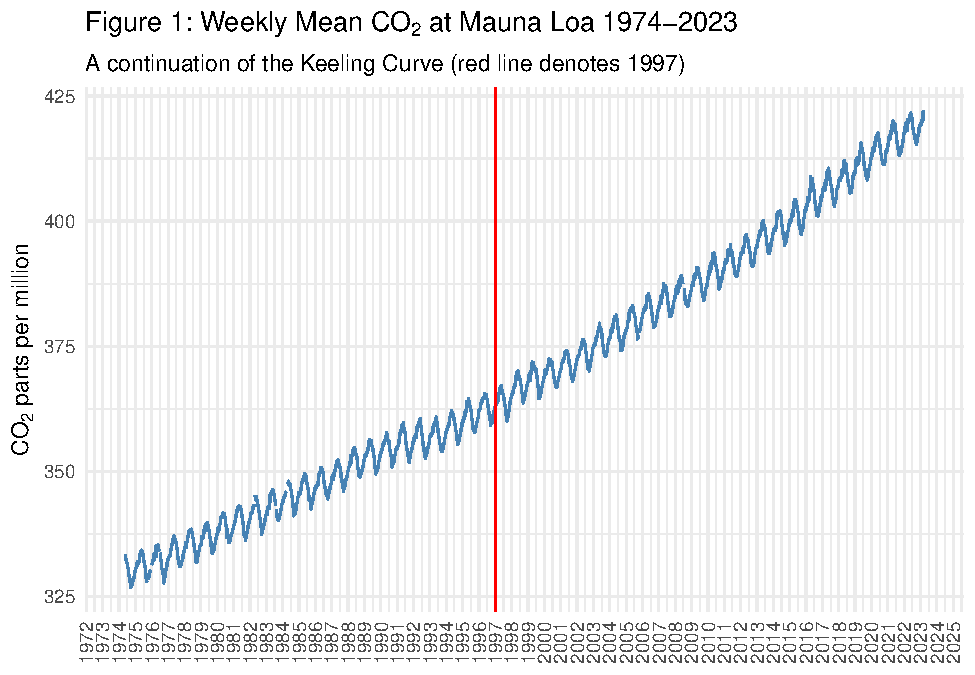
\includegraphics{co2_present_files/figure-latex/present time series-1.pdf}

From this time series, we observe a steady continuation of the Keeling
curve, with a continual increase in \(CO_{2}\) concentration (ppm) as
well as a notable seasonal component. The curve of the overall
increasing \(CO_{2}\) concentration, compared to data prior to 1997,
does appear to be increasing at a slightly higher rate than what was
previously observed.

To more carefully compare the distrbution and autocorrelation aspects of
this times series, we conducted further analysis, as shown below in
Figure 2.

\begin{verbatim}
## `stat_bin()` using `bins = 30`. Pick better value with `binwidth`.
\end{verbatim}

\begin{verbatim}
## Warning: Removed 18 rows containing non-finite values (`stat_bin()`).
\end{verbatim}

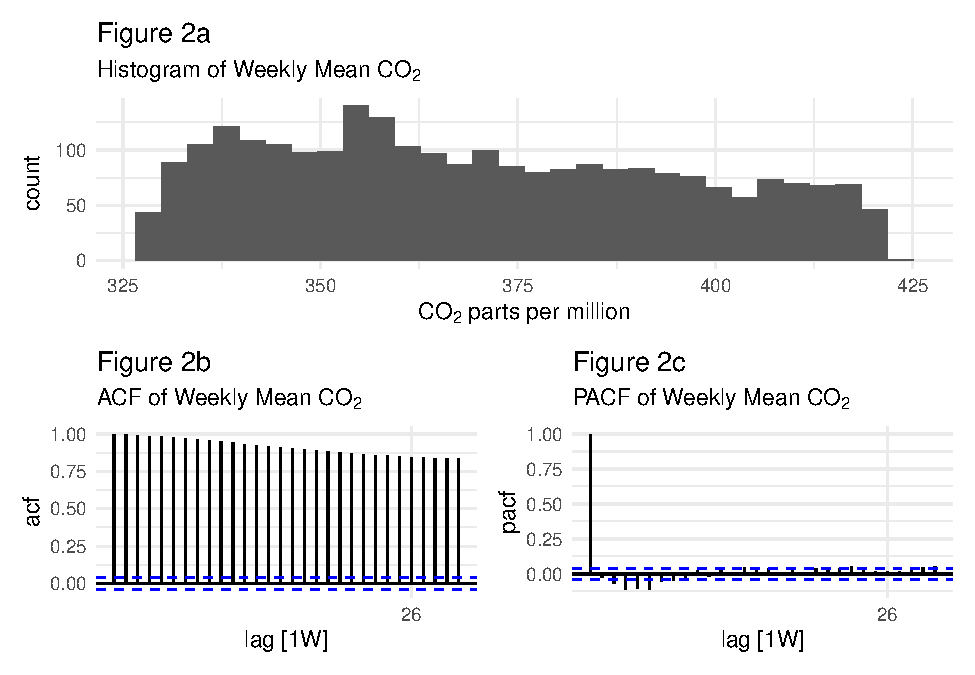
\includegraphics{co2_present_files/figure-latex/present histogram ACF PACF-1.pdf}

Figure 2 reveals that the present dataset recapitulates the behavior
observed in the 1997 dataset. Similar to what was seen in 1997, there is
a strong autocorrelation in \(CO_{2}\) concentration with very mild
decay, maintaining its strong correlation even after a lag of 30 weeks
(Fig 2b). The partial autocorrelation, PACF plot, reveals a first
correlation of almost 1 and some cyclical correlations that may
correspond to the seasonality of the data (Fib 2c). Taken together, this
analysis suggests that there is a seasonal and potentially
autoregressive component to the data.

\hypertarget{models-and-forecasts}{%
\section{Models and Forecasts}\label{models-and-forecasts}}

Through our exploratory data analysis, we found that our weekly data
from 1974-2022 appears to behave very similarly to the data that was
analyzed in 1997. Stemming from this analysis, we move to specifically
evaluating the best linear and ARIMA model from the 1997 report against
this newer dataset.

\hypertarget{comparing-1997-linear-models}{%
\subsection{Comparing 1997 Linear
Models}\label{comparing-1997-linear-models}}

To begin, we compared the best linear model from the 1997 report. In
that report, we assessed four different models and determined that the
quadratic model with a seasonal adjustment component most accurately
described the data up to 1997. To compare this model, we forecasted this
model 25 years in the future to encompass 2023, and graphed it against
our current dataset, shown below in Figure 3.

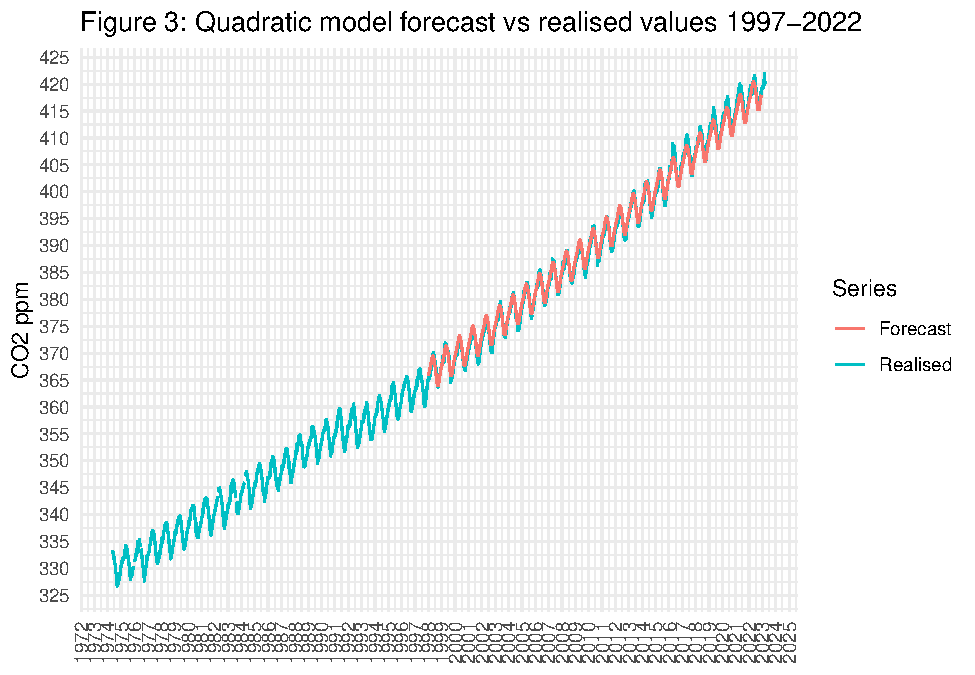
\includegraphics{co2_present_files/figure-latex/Compare against the realised values QUAD-1.pdf}

Figure 3 reveals that the quadratic with seasonality model forecast
fairly accurately predicts the actual data from 1997-2022. Up until
about 2016, the 1997 model does seem to routinely over-predict the
trough \(CO_{2}\) values per yearand after 2016, the 1997 quadratic with
seasonality model routinely under-predicts the peak \(CO_{2}\) values
per year. This suggests that while the quadratic model fits the data
fairly closely, a model that combines several localized trends might
better capture the data than a single overarching model.

\hypertarget{comparing-1997-arima-models}{%
\subsection{Comparing 1997 ARIMA
Models}\label{comparing-1997-arima-models}}

In addition to the linear model, the 1997 report also fit an ARIMA model
to the Keeling Curve \(CO_{2}\) data. We therefore wanted to
additionally evaluate how well that ARIMA model,
ARIMA(0,1,3)(0,1,1){[}12{]}, recapitulated the realized \(CO_{2}\)
concentrations from 1997-2022 (Figure 4 below).

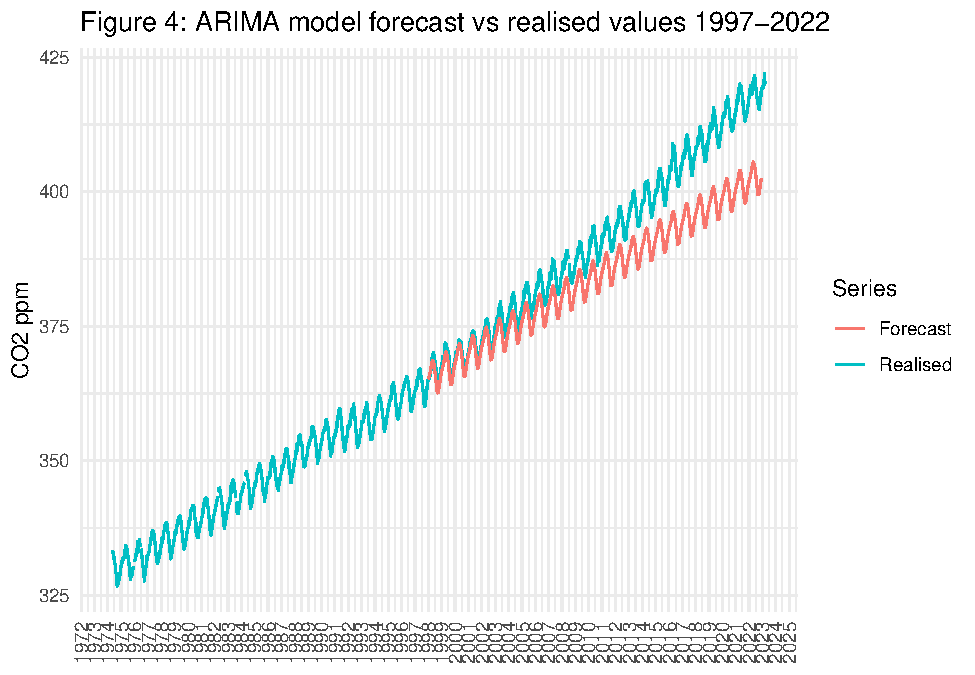
\includegraphics{co2_present_files/figure-latex/Compare against the realised values ARIMA-1.pdf}

As evident from Figure 4, the 1997 ARIMA model poorly predicted the
\(CO_{2}\) concentrations from 1997-2022, especially compared to the
quadratic with seasonality model also developed in 1997. From visual
inspection, the 1997 ARIMA model predicted a linearly increasing Keeling
Curve, rather than the quadratic process demonstrated in the previous
model. Because the \(CO_{2}\) concentration trends does appear to
increase more each year post 1997, following a quadratic pattern more
than a linear pattern, the ARIMA model consistently and more drastically
underpredicted \(CO_{2}\) concentrations at all points throughout the
year post 1997.

\hypertarget{evaluation-of-1997-forecasts}{%
\subsection{Evaluation of 1997
Forecasts}\label{evaluation-of-1997-forecasts}}

To more formally compare the 1997 models, we evaluate the specific
accuracy of several forecasts generated in the 1997 report to assess how
closely they matched the current realized data. In 1997, we predicted
the first and final times \(CO_{2}\) concetnration levels would reach
420 ppm and 500 ppm. We also evaluated predicted \(CO_{2}\)
concentrations in the year 2100. As of the date of writing this report
(published March 2023), we have not yet crossed the 500 ppm threshold
nor have data on \(CO_{2}\) in the year 2100, however we have already
reached 420 ppm.

In the 1997 report, 420 ppm predictions were generated using the
ARIMA(0,1,3)(0,1,1){[}12{]} model only, because at the time that model
was assessed to best recapitulate the data. In the 1997 report,
\(CO_{2}\) concentrations was predicted to first cross the 420 ppm
threshold in April 2032, however, the current data reveals that we
actually first crossed the 420 ppm threshold in May 2021 according to
the weekly data and April 2022 when the current data is aggregated
monthly, a full 10-11 years prior to the 1997 ARIMA model estimate. As
discussed above, the 1997 ARIMA model severely underestimated the growth
rate of the Keeling Curve past 1997. In contrast and as can be shown
below in Figure 5 (the blue horizontal line corresponds to the 420 ppm
threshold), the quadratic model with seasonality developed in the 1997
report predicted a May 2022 estimate for monthly mean \(CO_{2}\)
concentration, which compared to the ARIMA model is a much more accurate
forecast.

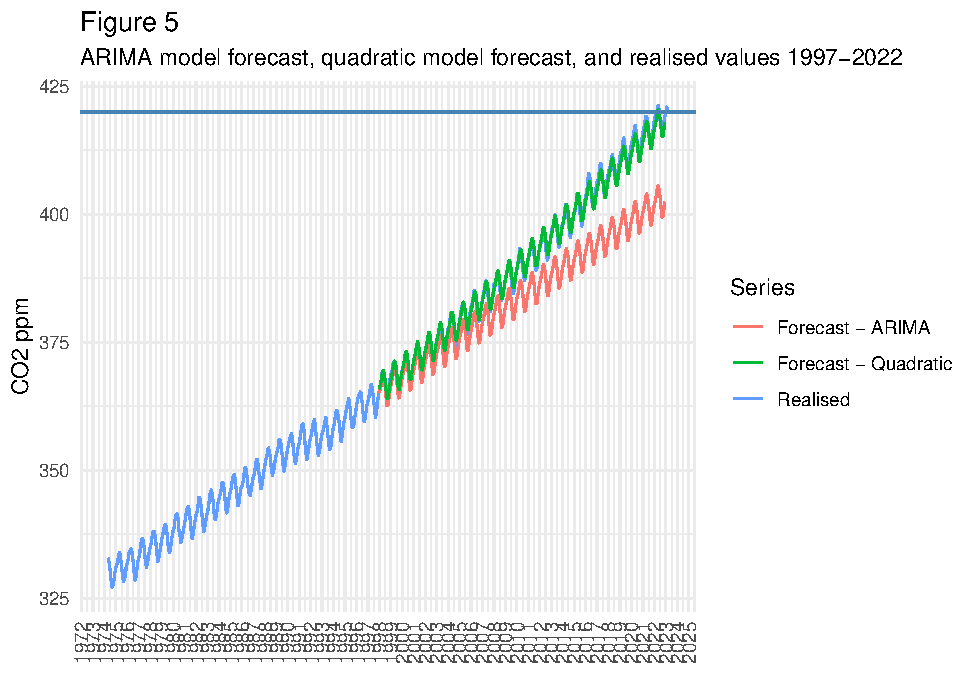
\includegraphics{co2_present_files/figure-latex/Plot the monthly series against the forecast-1.pdf}

To more rigorously compare the accuracy of the two models, we assessed
numerous accuracy measures for each 1997 model against the aggregated
monthly average data used in the this report, comparing forecasted
accuracy from 1997-2022. The results are summarized in Table 1 (below)
and reveal that across each metric (mean error (ME), root mean squared
error (RMSE), mean absolute error (MAE), mean percentage error (MPE),
mean absolute percentage error (MAPE), mean absolute scaled error
(MASE), root mean squared scaled error (RMSSE), and autocorrelation
errors at lag 1 (ACF1)), the 1997 quadratic with seasonality model
outperformed the 1997 ARIMA model.

\begin{longtable}[]{@{}
  >{\raggedright\arraybackslash}p{(\columnwidth - 16\tabcolsep) * \real{0.5000}}
  >{\raggedleft\arraybackslash}p{(\columnwidth - 16\tabcolsep) * \real{0.0625}}
  >{\raggedleft\arraybackslash}p{(\columnwidth - 16\tabcolsep) * \real{0.0625}}
  >{\raggedleft\arraybackslash}p{(\columnwidth - 16\tabcolsep) * \real{0.0521}}
  >{\raggedleft\arraybackslash}p{(\columnwidth - 16\tabcolsep) * \real{0.0729}}
  >{\raggedleft\arraybackslash}p{(\columnwidth - 16\tabcolsep) * \real{0.0625}}
  >{\raggedleft\arraybackslash}p{(\columnwidth - 16\tabcolsep) * \real{0.0625}}
  >{\raggedleft\arraybackslash}p{(\columnwidth - 16\tabcolsep) * \real{0.0625}}
  >{\raggedleft\arraybackslash}p{(\columnwidth - 16\tabcolsep) * \real{0.0625}}@{}}
\caption{1997 Model Forecasting Accuracy 1997-2022}\tabularnewline
\toprule()
\begin{minipage}[b]{\linewidth}\raggedright
.model
\end{minipage} & \begin{minipage}[b]{\linewidth}\raggedleft
ME
\end{minipage} & \begin{minipage}[b]{\linewidth}\raggedleft
RMSE
\end{minipage} & \begin{minipage}[b]{\linewidth}\raggedleft
MAE
\end{minipage} & \begin{minipage}[b]{\linewidth}\raggedleft
MPE
\end{minipage} & \begin{minipage}[b]{\linewidth}\raggedleft
MAPE
\end{minipage} & \begin{minipage}[b]{\linewidth}\raggedleft
MASE
\end{minipage} & \begin{minipage}[b]{\linewidth}\raggedleft
RMSSE
\end{minipage} & \begin{minipage}[b]{\linewidth}\raggedleft
ACF1
\end{minipage} \\
\midrule()
\endfirsthead
\toprule()
\begin{minipage}[b]{\linewidth}\raggedright
.model
\end{minipage} & \begin{minipage}[b]{\linewidth}\raggedleft
ME
\end{minipage} & \begin{minipage}[b]{\linewidth}\raggedleft
RMSE
\end{minipage} & \begin{minipage}[b]{\linewidth}\raggedleft
MAE
\end{minipage} & \begin{minipage}[b]{\linewidth}\raggedleft
MPE
\end{minipage} & \begin{minipage}[b]{\linewidth}\raggedleft
MAPE
\end{minipage} & \begin{minipage}[b]{\linewidth}\raggedleft
MASE
\end{minipage} & \begin{minipage}[b]{\linewidth}\raggedleft
RMSSE
\end{minipage} & \begin{minipage}[b]{\linewidth}\raggedleft
ACF1
\end{minipage} \\
\midrule()
\endhead
arima013011 & 6.974 & 8.496 & 6.97 & 1.737 & 1.737 & 4.727 & 5.382 &
0.985 \\
TSLM(value \textasciitilde{} trend() + I(trend()\^{}2) + season()) &
0.006 & 0.919 & 0.72 & -0.003 & 0.183 & 0.488 & 0.582 & 0.837 \\
\bottomrule()
\end{longtable}

\hypertarget{training-new-models-based-on-present-data}{%
\section{Training New Models Based on Present
Data}\label{training-new-models-based-on-present-data}}

\hypertarget{arima-models}{%
\subsection{ARIMA Models}\label{arima-models}}

Since we have conducted a thorough analysis of the models developed in
the 1997 report, we now wanted to devise updated models on this more
granular and recent \(CO_{2}\) concentration data. In order to do this,
we seasonally adjusted the weekly data, and split both the seasonally
adjusted (SA) and non-seasonally adjusted (NSA) data into training and
test sets. Because we are working with time series data, our test sets
were comprised of the most recent 2 years of weekly \(CO_{2}\)
concentrations (2020-2022). We fitted both SA and NSA training data sets
to ARIMA models. Before fitting ARIMA models, we took the first
difference of the data to remove the increasing trend and evaluated
whether or not the weekly data was stationary post differencing (since
stationarity is an assumption of ARIMA models).

\begin{verbatim}
## 
##  Phillips-Perron Unit Root Test
## 
## data:  train.diff.sa$diff[-1]
## Dickey-Fuller = -108, Truncation lag parameter = 8, p-value = 0.01
\end{verbatim}

\begin{verbatim}
## 
##  Augmented Dickey-Fuller Test
## 
## data:  train.diff.sa$diff[-1]
## Dickey-Fuller = -19, Lag order = 13, p-value = 0.01
## alternative hypothesis: stationary
\end{verbatim}

As shown above, using both the Phillips-Perron Unit Root Test and
Augemented Dickey-Fuller Test we reject the null hypothesis that the
first difference of the SA weekly \(CO_{2}\) concentration data is
non-stationary.

\begin{verbatim}
## 
##  Phillips-Perron Unit Root Test
## 
## data:  train.diff.nsa$diff[-1]
## Dickey-Fuller = -53, Truncation lag parameter = 8, p-value = 0.01
\end{verbatim}

\begin{verbatim}
## 
##  Augmented Dickey-Fuller Test
## 
## data:  train.diff.nsa$diff[-1]
## Dickey-Fuller = -16, Lag order = 13, p-value = 0.01
## alternative hypothesis: stationary
\end{verbatim}

Similarly, using both the Phillips-Perron Unit Root Test and Augemented
Dickey-Fuller Test we also reject the null hypothesis that the first
difference of the NSA weekly \(CO_{2}\) concentration data is
non-stationary. We therefore call the first difference of both datasets
stationary processes and can proceed to fit ARIMA models.

\begin{verbatim}
## Series: ppm 
## Model: ARIMA(1,0,1)(1,1,0)[52] w/ drift 
## 
## Coefficients:
##          ar1      ma1     sar1  constant
##       0.9838  -0.7132  -0.4967    0.0446
## s.e.  0.0044   0.0208   0.0179    0.0029
## 
## sigma^2 estimated as 0.2571:  log likelihood=-1757
## AIC=3524   AICc=3524   BIC=3553
\end{verbatim}

\begin{verbatim}
## Series: ppm 
## Model: ARIMA(1,0,1)(1,1,0)[52] w/ drift 
## 
## Coefficients:
##          ar1      ma1     sar1  constant
##       0.9838  -0.7132  -0.4967    0.0446
## s.e.  0.0044   0.0208   0.0179    0.0029
## 
## sigma^2 estimated as 0.2571:  log likelihood=-1757
## AIC=3524   AICc=3524   BIC=3553
\end{verbatim}

\begin{verbatim}
## Series: season_adjust 
## Model: ARIMA(0,1,2)(1,0,0)[52] w/ drift 
## 
## Coefficients:
##           ma1      ma2     sar1  constant
##       -0.6127  -0.1583  -0.2323    0.0429
## s.e.   0.0199   0.0195   0.0202    0.0017
## 
## sigma^2 estimated as 0.1265:  log likelihood=-916
## AIC=1841   AICc=1841   BIC=1870
\end{verbatim}

\begin{verbatim}
## Series: season_adjust 
## Model: ARIMA(0,1,3)(2,0,0)[52] w/ drift 
## 
## Coefficients:
##           ma1      ma2      ma3     sar1     sar2  constant
##       -0.6033  -0.1430  -0.0095  -0.2882  -0.2660    0.0546
## s.e.   0.0204   0.0228   0.0196   0.0198   0.0201    0.0017
## 
## sigma^2 estimated as 0.1174:  log likelihood=-848
## AIC=1711   AICc=1711   BIC=1751
\end{verbatim}

For the NSA data, we fit two ARMIA models, ARIMA(1,0,1)(1,1,0){[}52{]}
based on the best (lowest) AIC (AIC = 3524) and
ARIMA(1,0,2)(1,1,0){[}52{]} based on the best (lowest) BIC (BIC = 3423)
from all permutations of ARIMA models with up to 10 autoregressive
processes, 2 unit roots differences, 10 moving average processes, and
the equivalent in seasonality components. We used similar techniques to
fit the SA data, and found that the same ARIMA model,
ARIMA(0,1,2)(1,0,0){[}52{]}, had the lowest AIC (AIC = 1841) and BIC
(BIC = 1870) for the SA data (model shown below).

For each of these models, we evaluated the model accuracy against the
training (in-sample) and test (out-sample) data sets.

\hypertarget{evaluating-accuracy}{%
\subsubsection{Evaluating accuracy}\label{evaluating-accuracy}}

To evaluate the ARIMA models, we first assessed each model (the best
model via AIC or BIC for either the NSA or SA data sets) accuracy
against the training data provided, which is described in Table 2 below.

\begin{longtable}[]{@{}
  >{\raggedright\arraybackslash}p{(\columnwidth - 22\tabcolsep) * \real{0.3333}}
  >{\raggedright\arraybackslash}p{(\columnwidth - 22\tabcolsep) * \real{0.0381}}
  >{\raggedright\arraybackslash}p{(\columnwidth - 22\tabcolsep) * \real{0.0667}}
  >{\raggedright\arraybackslash}p{(\columnwidth - 22\tabcolsep) * \real{0.0857}}
  >{\raggedleft\arraybackslash}p{(\columnwidth - 22\tabcolsep) * \real{0.0667}}
  >{\raggedleft\arraybackslash}p{(\columnwidth - 22\tabcolsep) * \real{0.0571}}
  >{\raggedleft\arraybackslash}p{(\columnwidth - 22\tabcolsep) * \real{0.0571}}
  >{\raggedleft\arraybackslash}p{(\columnwidth - 22\tabcolsep) * \real{0.0667}}
  >{\raggedleft\arraybackslash}p{(\columnwidth - 22\tabcolsep) * \real{0.0571}}
  >{\raggedleft\arraybackslash}p{(\columnwidth - 22\tabcolsep) * \real{0.0571}}
  >{\raggedleft\arraybackslash}p{(\columnwidth - 22\tabcolsep) * \real{0.0571}}
  >{\raggedleft\arraybackslash}p{(\columnwidth - 22\tabcolsep) * \real{0.0571}}@{}}
\caption{Evaluating ARIMA model accuracy for present data (Training
Data)}\tabularnewline
\toprule()
\begin{minipage}[b]{\linewidth}\raggedright
model
\end{minipage} & \begin{minipage}[b]{\linewidth}\raggedright
IC
\end{minipage} & \begin{minipage}[b]{\linewidth}\raggedright
.model
\end{minipage} & \begin{minipage}[b]{\linewidth}\raggedright
.type
\end{minipage} & \begin{minipage}[b]{\linewidth}\raggedleft
ME
\end{minipage} & \begin{minipage}[b]{\linewidth}\raggedleft
RMSE
\end{minipage} & \begin{minipage}[b]{\linewidth}\raggedleft
MAE
\end{minipage} & \begin{minipage}[b]{\linewidth}\raggedleft
MPE
\end{minipage} & \begin{minipage}[b]{\linewidth}\raggedleft
MAPE
\end{minipage} & \begin{minipage}[b]{\linewidth}\raggedleft
MASE
\end{minipage} & \begin{minipage}[b]{\linewidth}\raggedleft
RMSSE
\end{minipage} & \begin{minipage}[b]{\linewidth}\raggedleft
ACF1
\end{minipage} \\
\midrule()
\endfirsthead
\toprule()
\begin{minipage}[b]{\linewidth}\raggedright
model
\end{minipage} & \begin{minipage}[b]{\linewidth}\raggedright
IC
\end{minipage} & \begin{minipage}[b]{\linewidth}\raggedright
.model
\end{minipage} & \begin{minipage}[b]{\linewidth}\raggedright
.type
\end{minipage} & \begin{minipage}[b]{\linewidth}\raggedleft
ME
\end{minipage} & \begin{minipage}[b]{\linewidth}\raggedleft
RMSE
\end{minipage} & \begin{minipage}[b]{\linewidth}\raggedleft
MAE
\end{minipage} & \begin{minipage}[b]{\linewidth}\raggedleft
MPE
\end{minipage} & \begin{minipage}[b]{\linewidth}\raggedleft
MAPE
\end{minipage} & \begin{minipage}[b]{\linewidth}\raggedleft
MASE
\end{minipage} & \begin{minipage}[b]{\linewidth}\raggedleft
RMSSE
\end{minipage} & \begin{minipage}[b]{\linewidth}\raggedleft
ACF1
\end{minipage} \\
\midrule()
\endhead
ARIMA(1,0,1)(1,1,0){[}52{]} (NSA data) & AIC & auto & Training & 0.008 &
0.501 & 0.382 & 0.002 & 0.104 & 0.208 & 0.249 & 0.127 \\
ARIMA(0,1,2)(1,0,0){[}52{]} (SA data) & AIC & auto & Training & -0.001 &
0.355 & 0.269 & -0.001 & 0.073 & 0.148 & 0.178 & 0.003 \\
ARIMA(1,0,1)(1,1,0){[}52{]} (NSA data) & BIC & auto & Training & 0.008 &
0.501 & 0.382 & 0.002 & 0.104 & 0.208 & 0.249 & 0.127 \\
ARIMA(0,1,2)(1,0,0){[}52{]} (SA data) & BIC & auto & Training & -0.001 &
0.342 & 0.259 & -0.001 & 0.070 & 0.141 & 0.170 & 0.000 \\
\bottomrule()
\end{longtable}

Based on the in-sample accuracy comparisons, for non seasonally adjusted
data, we chose the ARIMA(1,0,4)(1,1,0) model because it had slightly
better (lower) root mean squared error and ACF1 compared to the other
ARIMA model (ARIMA(1,0,2)(1,1,0)). For the seasonally adjusted data, we
only had one ARIMA model, ARIMA(0,1,2)(1,0,0), and use that model for
out-sample evaluation.

To evaluate our chosen ARIMA models further, we used each model (for NSA
and SA sata respectively) to forecast 2 years in the future (2020-2022)
and compared the accuracy of each model against our test data sets (both
for NSA and SA data). These results are described below in Table 3.

\begin{longtable}[]{@{}
  >{\raggedright\arraybackslash}p{(\columnwidth - 14\tabcolsep) * \real{0.3582}}
  >{\raggedright\arraybackslash}p{(\columnwidth - 14\tabcolsep) * \real{0.1045}}
  >{\raggedleft\arraybackslash}p{(\columnwidth - 14\tabcolsep) * \real{0.0896}}
  >{\raggedleft\arraybackslash}p{(\columnwidth - 14\tabcolsep) * \real{0.0896}}
  >{\raggedleft\arraybackslash}p{(\columnwidth - 14\tabcolsep) * \real{0.0896}}
  >{\raggedleft\arraybackslash}p{(\columnwidth - 14\tabcolsep) * \real{0.0896}}
  >{\raggedleft\arraybackslash}p{(\columnwidth - 14\tabcolsep) * \real{0.0896}}
  >{\raggedleft\arraybackslash}p{(\columnwidth - 14\tabcolsep) * \real{0.0896}}@{}}
\caption{Present ARIMA Model Forecasting Accuracy
2020-2022}\tabularnewline
\toprule()
\begin{minipage}[b]{\linewidth}\raggedright
data
\end{minipage} & \begin{minipage}[b]{\linewidth}\raggedright
.model
\end{minipage} & \begin{minipage}[b]{\linewidth}\raggedleft
ME
\end{minipage} & \begin{minipage}[b]{\linewidth}\raggedleft
RMSE
\end{minipage} & \begin{minipage}[b]{\linewidth}\raggedleft
MAE
\end{minipage} & \begin{minipage}[b]{\linewidth}\raggedleft
MPE
\end{minipage} & \begin{minipage}[b]{\linewidth}\raggedleft
MAPE
\end{minipage} & \begin{minipage}[b]{\linewidth}\raggedleft
ACF1
\end{minipage} \\
\midrule()
\endfirsthead
\toprule()
\begin{minipage}[b]{\linewidth}\raggedright
data
\end{minipage} & \begin{minipage}[b]{\linewidth}\raggedright
.model
\end{minipage} & \begin{minipage}[b]{\linewidth}\raggedleft
ME
\end{minipage} & \begin{minipage}[b]{\linewidth}\raggedleft
RMSE
\end{minipage} & \begin{minipage}[b]{\linewidth}\raggedleft
MAE
\end{minipage} & \begin{minipage}[b]{\linewidth}\raggedleft
MPE
\end{minipage} & \begin{minipage}[b]{\linewidth}\raggedleft
MAPE
\end{minipage} & \begin{minipage}[b]{\linewidth}\raggedleft
ACF1
\end{minipage} \\
\midrule()
\endhead
Non-seasonally adjusted & auto & 0.277 & 0.608 & 0.507 & 0.066 & 0.121 &
0.252 \\
Seasonally adjusted & auto & 0.858 & 1.015 & 0.885 & 0.205 & 0.212 &
0.439 \\
\bottomrule()
\end{longtable}

\hypertarget{polynomial-model}{%
\subsection{Polynomial Model}\label{polynomial-model}}

\begin{verbatim}
## Series: season_adjust 
## Model: TSLM 
## 
## Residuals:
##    Min     1Q Median     3Q    Max 
## -2.471 -0.644 -0.126  0.634  2.682 
## 
## Coefficients:
##              Estimate Std. Error t value Pr(>|t|)    
## (Intercept)  3.31e+02   5.19e-02    6376   <2e-16 ***
## trend()      2.23e-02   9.84e-05     226   <2e-16 ***
## I(trend()^2) 4.95e-06   3.91e-08     127   <2e-16 ***
## ---
## Signif. codes:  0 '***' 0.001 '**' 0.01 '*' 0.05 '.' 0.1 ' ' 1
## 
## Residual standard error: 0.852 on 2431 degrees of freedom
## Multiple R-squared: 0.999,   Adjusted R-squared: 0.999
## F-statistic: 9.83e+05 on 2 and 2431 DF, p-value: <2e-16
\end{verbatim}

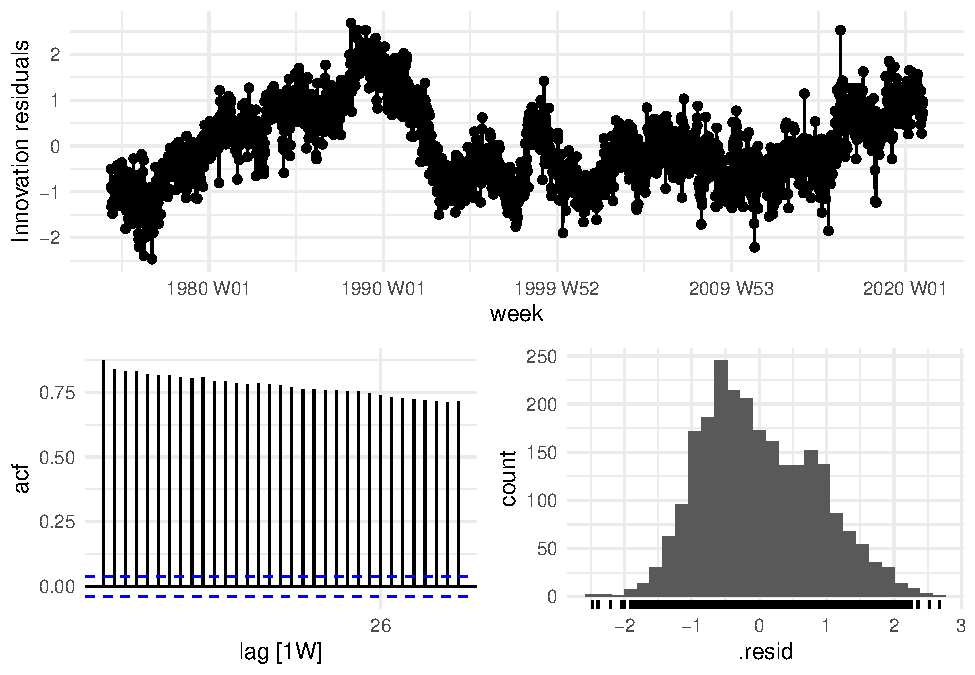
\includegraphics{co2_present_files/figure-latex/Poly-time trend model to SA-1.pdf}

\hypertarget{evaluating-accuracy-1}{%
\subsubsection{Evaluating Accuracy}\label{evaluating-accuracy-1}}

\begin{verbatim}
## # A tibble: 1 x 10
##   .model                   .type    ME  RMSE   MAE   MPE  MAPE  MASE RMSSE  ACF1
##   <chr>                    <chr> <dbl> <dbl> <dbl> <dbl> <dbl> <dbl> <dbl> <dbl>
## 1 TSLM(season_adjust ~ tr~ Test  0.680 0.853 0.723 0.163 0.173   NaN   NaN 0.432
\end{verbatim}

\hypertarget{how-bad-could-it-get}{%
\section{How Bad Could It Get?}\label{how-bad-could-it-get}}

\hypertarget{points-task-part-6b-how-bad-could-it-get}{%
\subsection{(3 points) Task Part 6b: How bad could it
get?}\label{points-task-part-6b-how-bad-could-it-get}}

With the non-seasonally adjusted data series, generate predictions for
when atmospheric CO2 is expected to be at 420 ppm and 500 ppm levels for
the first and final times (consider prediction intervals as well as
point estimates in your answer). Generate a prediction for atmospheric
CO2 levels in the year 2122. How confident are you that these will be
accurate predictions?

\begin{longtable}[]{@{}
  >{\raggedleft\arraybackslash}p{(\columnwidth - 12\tabcolsep) * \real{0.1000}}
  >{\raggedright\arraybackslash}p{(\columnwidth - 12\tabcolsep) * \real{0.1286}}
  >{\raggedleft\arraybackslash}p{(\columnwidth - 12\tabcolsep) * \real{0.0857}}
  >{\raggedleft\arraybackslash}p{(\columnwidth - 12\tabcolsep) * \real{0.1714}}
  >{\raggedleft\arraybackslash}p{(\columnwidth - 12\tabcolsep) * \real{0.1714}}
  >{\raggedleft\arraybackslash}p{(\columnwidth - 12\tabcolsep) * \real{0.1714}}
  >{\raggedleft\arraybackslash}p{(\columnwidth - 12\tabcolsep) * \real{0.1714}}@{}}
\caption{Predictions on crossing the 420 and 500 CO2 ppm}\tabularnewline
\toprule()
\begin{minipage}[b]{\linewidth}\raggedleft
target
\end{minipage} & \begin{minipage}[b]{\linewidth}\raggedright
week
\end{minipage} & \begin{minipage}[b]{\linewidth}\raggedleft
.mean
\end{minipage} & \begin{minipage}[b]{\linewidth}\raggedleft
ci.80.lower
\end{minipage} & \begin{minipage}[b]{\linewidth}\raggedleft
ci.80.upper
\end{minipage} & \begin{minipage}[b]{\linewidth}\raggedleft
ci.95.lower
\end{minipage} & \begin{minipage}[b]{\linewidth}\raggedleft
ci.95.upper
\end{minipage} \\
\midrule()
\endfirsthead
\toprule()
\begin{minipage}[b]{\linewidth}\raggedleft
target
\end{minipage} & \begin{minipage}[b]{\linewidth}\raggedright
week
\end{minipage} & \begin{minipage}[b]{\linewidth}\raggedleft
.mean
\end{minipage} & \begin{minipage}[b]{\linewidth}\raggedleft
ci.80.lower
\end{minipage} & \begin{minipage}[b]{\linewidth}\raggedleft
ci.80.upper
\end{minipage} & \begin{minipage}[b]{\linewidth}\raggedleft
ci.95.lower
\end{minipage} & \begin{minipage}[b]{\linewidth}\raggedleft
ci.95.upper
\end{minipage} \\
\midrule()
\endhead
420 & 2022 W13 & 421 & 419 & 422 & 419 & 422 \\
420 & 2025 W40 & 421 & 418 & 423 & 417 & 424 \\
500 & 2065 W09 & 500 & 492 & 508 & 488 & 512 \\
500 & 2068 W35 & 500 & 492 & 508 & 488 & 513 \\
\bottomrule()
\end{longtable}

We now show predictions for the year 2122:

\begin{longtable}[]{@{}lrrrrr@{}}
\caption{Predictions for the year 2122}\tabularnewline
\toprule()
week & .mean & ci.80.lower & ci.80.upper & ci.95.lower & ci.95.upper \\
\midrule()
\endfirsthead
\toprule()
week & .mean & ci.80.lower & ci.80.upper & ci.95.lower & ci.95.upper \\
\midrule()
\endhead
2122 W02 & 605 & 593 & 616 & 587 & 623 \\
2122 W03 & 605 & 593 & 617 & 587 & 623 \\
2122 W04 & 605 & 593 & 616 & 587 & 623 \\
2122 W05 & 604 & 592 & 616 & 586 & 622 \\
2122 W06 & 604 & 592 & 616 & 586 & 622 \\
2122 W07 & 604 & 592 & 615 & 586 & 621 \\
2122 W08 & 603 & 592 & 615 & 585 & 621 \\
2122 W09 & 603 & 591 & 614 & 585 & 620 \\
2122 W10 & 602 & 591 & 614 & 584 & 620 \\
2122 W11 & 601 & 590 & 613 & 584 & 619 \\
2122 W12 & 601 & 589 & 612 & 583 & 618 \\
2122 W13 & 601 & 589 & 612 & 583 & 618 \\
2122 W14 & 600 & 589 & 612 & 583 & 618 \\
2122 W15 & 600 & 588 & 611 & 582 & 618 \\
2122 W16 & 600 & 588 & 611 & 582 & 617 \\
2122 W17 & 599 & 587 & 611 & 581 & 617 \\
2122 W18 & 599 & 587 & 610 & 581 & 617 \\
2122 W19 & 599 & 587 & 610 & 581 & 617 \\
2122 W20 & 598 & 587 & 610 & 581 & 616 \\
2122 W21 & 598 & 587 & 610 & 581 & 616 \\
2122 W22 & 599 & 587 & 610 & 581 & 616 \\
2122 W23 & 599 & 587 & 610 & 581 & 616 \\
2122 W24 & 599 & 587 & 611 & 581 & 617 \\
2122 W25 & 599 & 587 & 611 & 581 & 617 \\
2122 W26 & 599 & 588 & 611 & 582 & 617 \\
2122 W27 & 600 & 589 & 612 & 582 & 618 \\
2122 W28 & 600 & 588 & 612 & 582 & 618 \\
2122 W29 & 601 & 589 & 613 & 583 & 619 \\
2122 W30 & 601 & 590 & 613 & 583 & 619 \\
2122 W31 & 601 & 589 & 613 & 583 & 619 \\
2122 W32 & 602 & 590 & 613 & 584 & 619 \\
2122 W33 & 602 & 590 & 614 & 584 & 620 \\
2122 W34 & 603 & 591 & 614 & 585 & 620 \\
2122 W35 & 603 & 591 & 614 & 585 & 621 \\
2122 W36 & 603 & 591 & 614 & 585 & 620 \\
2122 W37 & 604 & 592 & 615 & 586 & 621 \\
2122 W38 & 604 & 592 & 615 & 586 & 621 \\
2122 W39 & 604 & 592 & 616 & 586 & 622 \\
2122 W40 & 604 & 593 & 616 & 586 & 622 \\
2122 W41 & 604 & 592 & 615 & 586 & 621 \\
2122 W42 & 604 & 592 & 615 & 586 & 622 \\
2122 W43 & 604 & 592 & 615 & 586 & 622 \\
2122 W44 & 604 & 592 & 616 & 586 & 622 \\
2122 W45 & 604 & 592 & 616 & 586 & 622 \\
2122 W46 & 605 & 593 & 616 & 587 & 622 \\
2122 W47 & 605 & 593 & 617 & 587 & 623 \\
2122 W48 & 606 & 594 & 617 & 588 & 624 \\
2122 W49 & 606 & 594 & 617 & 588 & 624 \\
2122 W50 & 606 & 594 & 617 & 588 & 623 \\
2122 W51 & 606 & 595 & 618 & 589 & 624 \\
2122 W52 & 606 & 595 & 618 & 589 & 624 \\
2122 W53 & 607 & 595 & 618 & 589 & 625 \\
\bottomrule()
\end{longtable}

\hypertarget{conclusions}{%
\section{Conclusions}\label{conclusions}}

What to conclude is unclear.


\end{document}
